\chapter*[Introduction]{Introduction}
\addcontentsline{toc}{chapter}{Introduction}

The research and advancement of scientific knowledge can be very daunting, especially without a scientific background. Requirements such as a well-defined methodology, high data quality, and a strict revision process may present some barriers to the common citizen. However, with the recent advancement in technology \cite{newman2012future}, connectivity \cite{newman2012future} and interest in science by the public \cite{silvertown2009new}, there has been a rising trend in the general populace contributing to a special kind of science: Citizen Science \cite{mckinley2017citizen}.

Citizen science refers to research that engages nonprofessionals in the process of creating new scientific knowledge \cite{bonney2014next}. Referred to as citizen scientists; these nonprofessionals may participate in a variety of tasks ranging in complexity; from simple tasks such as data gathering or classification \cite{barker2013pascal}, to even complex ones such as solving algorithms \cite{cooper2010predicting}. They may act as contributors and collaborators, but can also have a more proactive role as a project leader \cite{robinson2018ten}.

Citizen science is not new, as it has existed for more than one century now. However, its reach was reduced, since it was mostly focused on ecological and environmental sciences. Some initiatives date back to 1890, such as the Cooperative Weather Service, where amateurs send collected weather data to the National Weather Service; and 1966, the North American Breeding Bird Survey with more than 670 publications referencing it, where nonprofessionals map avian species distribution throughout North America over time. This practice has shown a rise in (1) the number of citizen science projects \footnote{Extraction from \href{citizenscience.gov}{citizenscience.gov}, and Zooniverse.} (figure \ref{fig:growth-citizen-science-projects}) as well as (2) articles published on the topic \footnote{Query String: "citizen science" in Scholar Google, filtered by one year intervals} (as seen in figure \ref{fig:growth-publications}).

\pgfplotstableread[row sep=\\,col sep=&]{
    year & publications \\
    2010 & 2810 \\
    2011 & 2750 \\
    2012 & 5220 \\
    2013 & 6990 \\
    2014 & 9330 \\
    2015 & 11900 \\
    2016 & 14500 \\
    2017 & 15800 \\
    2018 & 20200 \\
    2019 & 18300 \\
}\publicationdata

\begin{figure}[!h]
    \centering
    \begin{tikzpicture}
        \begin{axis}[
                ybar,
                bar width=.5cm,
                width=\textwidth,
                height=.5\textwidth,
                legend style={at={(0, 10)}, anchor=north,legend columns=-1},
                symbolic x coords={2010,2011,2012,2013,2014,2015,2016,2017,2018,2019,2020},
                xtick=data,
                nodes near coords,
                nodes near coords align={vertical},
                ymin=0,ymax=25000,
                ylabel={publications},
                xlabel={years},
            ]
            \addplot table[x=year,y=publications]{\publicationdata};
        \end{axis}
    \end{tikzpicture}
    \caption{Growth of citizen science initiatives over time}
    \label{fig:growth-citizen-science-projects}
\end{figure}

\begin{figure}[!h]
    \centering
    \begin{tikzpicture}
        \begin{axis}[
                ybar,
                bar width=.5cm,
                width=\textwidth,
                height=.5\textwidth,
                legend style={at={(0, 10)}, anchor=north,legend columns=-1},
                symbolic x coords={2010,2011,2012,2013,2014,2015,2016,2017,2018,2019,2020},
                xtick=data,
                nodes near coords,
                nodes near coords align={vertical},
                ymin=0,ymax=25000,
                ylabel={publications},
                xlabel={years},
            ]
            \addplot table[x=year,y=publications]{\publicationdata};
        \end{axis}
    \end{tikzpicture}
    \caption{Growth of published peer-reviewed articles on citizen science}
    \label{fig:growth-publications}
\end{figure}

This research field could be classified into three categories, based on volunteer involvement \cite{follett2015analysis}: (1) Contributory, where participants contribute to data collection and sometimes help analyze and disseminate results \cite{bonney2009citizen}, (2) Collaborative, where citizens also analyze samples, design the study, interpret the data, draw conclusions and disseminate results \cite{faridani2009networked} and (3) Co-created, where they participate in all stages of the project, including defining questions, developing the hypotheses, drawing conclusions, discussing results and answering new questions \cite{hill2012notes}.

As to why would a citizen collaborate, there could be several reasons depending on the project itself: contribution to the advancement of science or the project, desire to learn, personal interests, entertainment, among others \cite{tinati2016because}. This poses an engagement challenge, since public participation is vital to the result of the research; and is one of the studies of citizen science theory \cite{bowser2013using}.

At the other end of the spectrum, scientists lead citizen science initiatives. They enlist amateurs to contribute to projects, but also devise validation techniques from the collected data. They are also central to the role of acquiring sponsors in the government scenario, many of which are important to the feasibility of these initiatives.

With the rise in interest from the public, this discipline is able to achieve otherwise impossible results. According to \cite{theobald2015global}, in 2014, 1.3 million volunteers participated in 388 research projects related to biodiversity alone, contributing up to \$2.5 billion of in-kind labor annually.

This is just one of the many examples showing the potential of Citizen Science. It also comes with the realization that the public represents a free source of labor, skills, computational power, and even finance \cite{silvertown2009new}. Such perception could implicate in ethical concerns depending on how the data is gathered or processed, but also on how should the nonprofessional be (if he is) rewarded. With these among other concerns, the European Citizen Science Association conceived the "Ten principles of citizen science" \cite{robinson2018ten}. They establish some key principles to follow as good practice when applying citizen science concepts to research. Many of the principles focus on the protection of citizen scientist rights, since those individuals deserve feedback, acknowledgment, and participation rights to the research.

One significant factor supporting this growth is the availability of technical tools for disseminating information about projects and gathering data from the public \cite{silvertown2009new}. The widespread use of smartphones allows scientists to develop platforms easily accessible to everyone. This is combined with advancements in software usability on these platforms, resulting in a better first time usage as well as recurring contributions. In some research topics, low-cost hardware is stimulating robust data collection with less resources, providing unprecedented opportunities for knowledge generation \cite{buytaert2014citizen}. Online citizen science platforms (such as Zooniverse) provide an easy gateway to participation in a diverse set of projects, and have a high number of contributors \footnote{2,221,469 extracted from \url{https://www.zooniverse.org/} at 13/01/2021}.

Citizen participation in platforms like Zooniverse is the key to breakthroughs in scientific outcomes. Therefore, many studies focus on public engagement and community sustainability \cite{aristeidou2017profiles}. In these online communities, there is a high attrition rate recorded (\cite{nov2011technology} \cite{ponciano2015finding}), as well as dabbling behaviour \cite{eveleigh2014designing} in participation, even though it is recognized that user engagement is a necessary ingredient in the success of virtual environments \cite{verhagen2015benefitting}. Besides many of the reasons a citizen would collaborate, the look and feel of the project itself could change perspective and interpretation on how would a nonprofessional engage with the initiative.

One of the many techniques to overcome these engagement obstacles is throughout the use of gamification \cite{bowser2013using}. It refers to the addition of game elements to enhance user experience and engagement within non-game applications. Tasks are made to look more like games, employing, for instance scoring and competition. They are common in the private sector and have spread to education, health, government, and science. A recent report on consumer entertainment shows that in the the past six months, four of every five United States customers have played a video game (figure \ref{fig:entertainment-report}), illustrating the relevance of the segment. DFC Intelligence also released its 2020 Dossier with statements that nearly half of 3.1 billion gamers play games on their smartphones only. Gamers represent a significant portion of the population, so by gamifying them, citizen science projects scientists have a larger reach to this community.

\begin{figure}[ht]
    \centering
    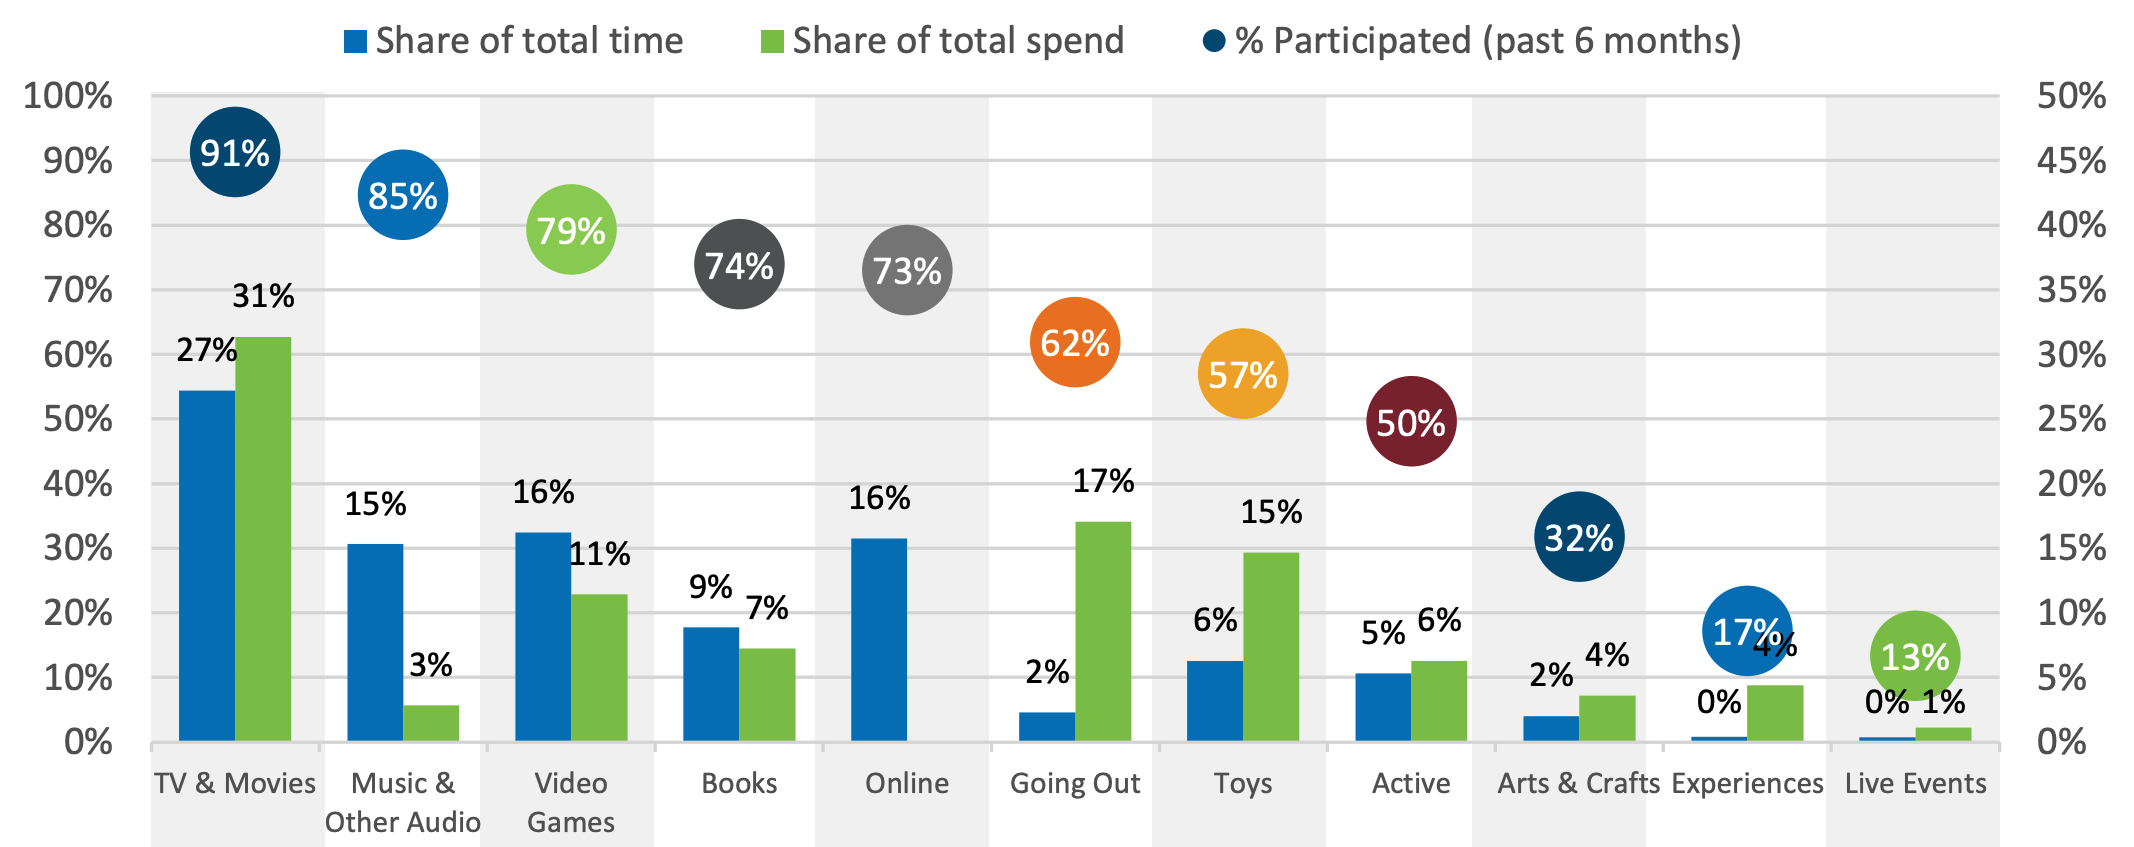
\includegraphics[width=\linewidth]{images/game.png}
    \caption{2020 Report on Entertainment Category Engagement; 79\% of the population is taken by gamers.\\ Source: 2020 Evolution of Entertainment / NPD Group}
    \label{fig:entertainment-report}
\end{figure}

Foldit, designed by researchers at the University of Washington, is a game in which gamers solve protein folding patterns, a central challenge in biochemistry, by virtually wiggling, shaking and pulling shapes to create small stable structures, as well as developing their own algorithms for solving protein folding \cite{bourzac2008enlisting}. This citizen science online game have had more than 800,000 registered players \footnote{As of 13/01/2021, \url{https://fold.it/portal/players}}, identified a potential target for HIV development, and redesigned a catalyst for the Diels-Alder reactions \cite{kreitmair2019citizen}. EyeWire is another example of the success of citizen science gamified environments. With more than 200,00 gamers from 145 countries, EyeWire allows users to map neurons in the retina, filling and extending areas missed by artificial intelligence \cite{kreitmair2019citizen}.

Once focused on ecological and environmental sciences, the citizen science practice has a much larger range now, covering topics such as linguistics \cite{svendsen2018dynamics}, astronomy \cite{marshall2015ideas}, hydrology \cite{buytaert2014citizen} etc. Out of these interest areas, one that could see further development with initiatives using citizen science is Natural Language Processing.

Natural language processing is a vast field that explores how computers can understand and manipulate human language in text or speech format. Researches in this area include (but are not limited to) sentiment analysis, sentence prediction, text translation, text-to-speech conversion, and speech recognition.

Also known as automatic speech recognition (ASR), computer speech recognition, or speech-to-text (STT), speech recognition is a field that studies the recognition and translation of spoken language into text by computers. It has been an intensive research area for decades, but has seen growth led by increased demand on ASR systems in the mobile environment \cite{yu2016automatic}, with virtual assistants, such as Alexa, Siri, Google Now.

Speech recognition is a class of machine learning that has seen many different approaches over time: stochastically modelling with Hidden Markov Models  \cite{gales2008application}, artificial intelligence learning with Neural Networks \cite{graves2013speech}, non-stochastical modelling \cite{burget2003nonrandomattr} and even hybrid approaches \cite{wang2020transformer} have been made to solve this complex interdisciplinary field.

However, these voice modeling strategies are highly dependant on the quality and quantity of data provided. Factors such as noisy speech data, nonhomogeneous recordings, different microphones within the same dataset, and even speech disorders could limit proper analysis, affect accuracy, and even change speech predictions \cite{wrong}. 

These voice datasets, also known as Speech Corpus (or Speech Corpora in plural), curate a collection of audio recordings of a spoken language. Some of them also have additional text files with transcriptions of the words spoken. Although they are widely found in the literature with robust recording procedures and analysis - such as TIMIT \cite{Lamel1992timmit}, DIRHA \cite{Ravanelli2016dirha} and the more recent \cite{chanchaochai2018globaltimit}) -, these datasets are structured in such a way that the speakers are individually selected. This could lead to bias problems \cite{bender2018data}, but also limits the number of voices recorded. Unfortunately, most speech corpora are recorded for the English language \cite{LeRouxVincent2014TRdatasets} and research is limited on the data quantity necessary to enable speech recognition systems and other voice applications.

To circumvent the quantity issue, some corpora are able to be constantly updated with user input. These online datasets can be accessed via web browser. Some examples are Vox Forge and Common Voice \cite{ardila2019common}. However, the former has poor user interface and little usage over time, and the latter has no structured analysis on bias mitigation, relying on crowdsourced information.

This work identifies the Citizen Science practice as a potential candidate to create a robust Speech Corpus for the low-resource Brazilian Portuguese language. A gamifyied application will be constructed to collect the data and engage users, applying data validation techniques to mitigate bias problems afterwards. The curated data will be published in a open-source platform to further research on speech recognition in this low-resource language.

\section*{Objective}

The main focus of this project lies in the construction and validation of a speech corpus for the brazilian portuguese language. The validated corpus and anonymized data will be available to the public.

\chapter{Method}

To achieve the aforementioned objective, this project will:

\begin{itemize}
    \item Research what characterizes a speech corpus in the literature;
    \item Create a list of phrases from which the public will read;
    \item Construct a application to record anonymized speech data;
    \item Add gamification elements to enhance public engagement;
    \item Validate recorded data and apply statistical methods to ensure data quality
    \item Publish dataset on open source platform
\end{itemize}

\section{Document structure}

This document is divided in 4 chapters:

\begin{itemize}
    \item Chapter 1 presents the context, motivation, and objective of the proposed research
    \item Chapter 2 details the background and foundation of all areas related to this research
    \item Chapter 3 presents related work on corpus creation
    \item Chapter 4 presents the systematic literature review to understand what characterizes a speech corpus
    \item Chapter 4 contains the proposed work to finish this research
\end{itemize}
